\uuid{aNdK}
\exo7id{7104}
\auteur{megy}
\organisation{exo7}
\datecreate{2017-01-21}
\isIndication{true}
\isCorrection{true}
\chapitre{Géométrie affine euclidienne}
\sousChapitre{Géométrie affine euclidienne du plan}

\contenu{
\texte{
% tags : rotation, translation, difficile
On considère un carré $ABCD$ et on place quatre points $E$, $F$, $G$, et $H$ sur les côtés de ce carré, en-dehors des sommets. Puis, on efface le carré. En considérant une rotation et une translation, reconstruire le carré.
}
\indication{Il suffit de construire une des droites d'appui du carré. Pour cela, il suffit de construire un deuxième point sur cette droite.}
\reponse{
Voici une solution dans une configuration \og générique\fg.

Commençons par analyser le problème. On suppose que $ABCD$ est direct et que $E\in [AB]$, $F \in [BC]$ etc.
Considérons la rotation de centre $O$ (le centre du carré), et d'angle $\pi/4$. L'image du segment $[EG]$ est un segment $[E'G']$, que l'on suppose distinct de $[FH]$. En fait, on suppose pour simplifier $E'\neq F$. Considérons alors la translation de vecteur $\overrightarrow{E'F}$. Elle envoie $G'$ sur un point $G''$ appartenant à la droite $(DA)$. Si on suppose que ce point est différent de $H$, alors on a $(DA) = (G''H)$. 

Voici comment obtenir le point $G''$. On construit la perpendiculaire à $(EG)$ passant par $F$, et sur cette droite, on place le point $G''$ tel que $FG''=EG$ et $(\overrightarrow{EG},\overrightarrow{FG''}) = \pi/2$. Ceci permet de tracer la droite $(HG'')$ c'est-à-dire $(AD)$.

\begin{center}
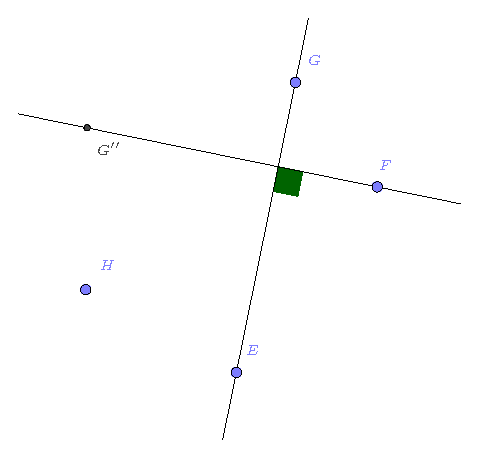
\includegraphics{../images/img007104-1}
\end{center}

On projette ensuite les points $E$ et $G$ sur cette droite, ce qui donne $A$ et $D$. On peut ensuite terminer la construction du carré.

Il existe d'autres solutions qui utilisent le théorème de l'angle au centre.
}
}
